 \section{The TEPX upgrade for Phase II HL-LHC}
\label{sec:tepx}

The High Luminosity (HL)-LHC will increase instantaneous luminosity to unprecedented value of $7.5 \times 10^{34} cm^{-2} s^{-1}$ which corresponds to 200 proton-proton collisions per bunch crossing (pileup). Run 2 pixel detector will not be able to handle the extreme radiation environment, resolve nearby particle tracks and operate properly to give a reliable estimate of the instantaneous luminosity for high pileup values. That is why it will be replaced by a new pixel detector which will be composed of three subdetectors: tracker barrel pixel detector (TBPX), tracker forward pixel detector (TFPX) and tracker endcap pixel detector (TEPX). TEPX will have better radiation tolerance, increased granularity, improved two-track separation, improved estimation of hit rate and statistical precision, extended tracking acceptance $|\eta|=4$ with Disk 4 Ring 1 operating as an independent luminometer \cite{Klein:2017nke}. \\


\subsection{TEPX detector for Phase II}

Tracker endcap pixel detector (TEPX) consists of four double disks per side (-Z and +Z) with each double disk containing five rings as shown in Fig. 25 having 20, 28, 36, 44 and 48 modules respectively. One double disk has four surfaces with +Z side containing modules with even module number in front layers (L1 $\&$ L2) and modules with odd module number in back layers (L3 $\&$ L4) from Ring 1 to Ring 4 and for Ring 5, modules with odd module number in front layers and modules with even module number in back layers as shown in Fig. 26. For -Z side, four surfaces contain modules with odd module number in front layer and modules with even module number in back layer from Ring 1 to Ring 4 and for Ring 5, modules with even module number in front layer and modules with odd module number in back layer. \\


\begin{figure}[H]
  \centering
  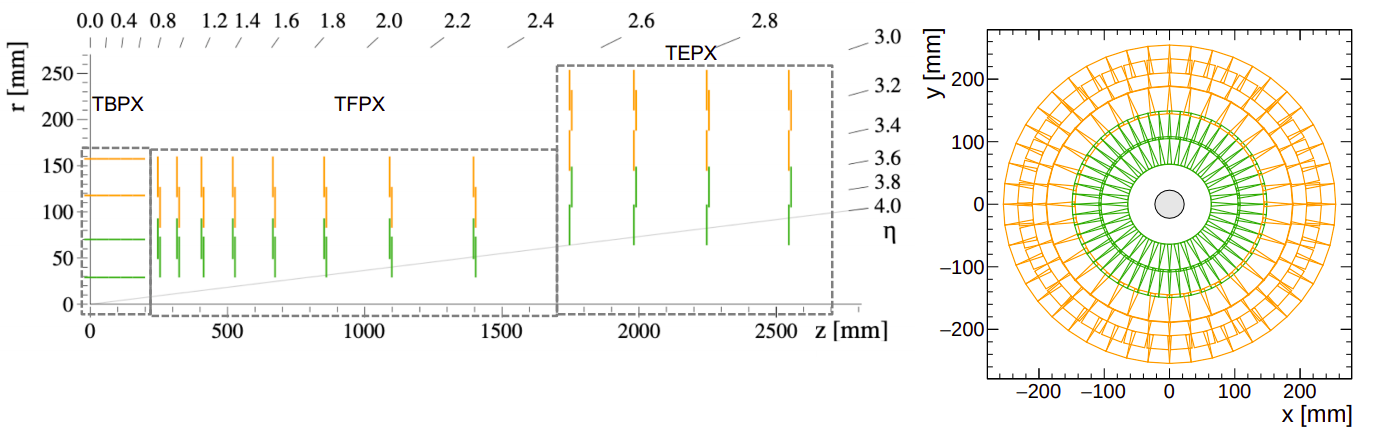
\includegraphics[width=1 \columnwidth]{./tepx_tt.png}
  \caption{ \onehalfspacing Left: A layout of the CMS Phase II inner tracker showing four TEPX disks, eight TFPX disks and four barrel layers. Right: Diagram showing one double disk of TEPX with five rings \cite{Klein:2017nke}.}
  \label{fig:CMS}
\end{figure}


\begin{figure}[H]
  \centering
  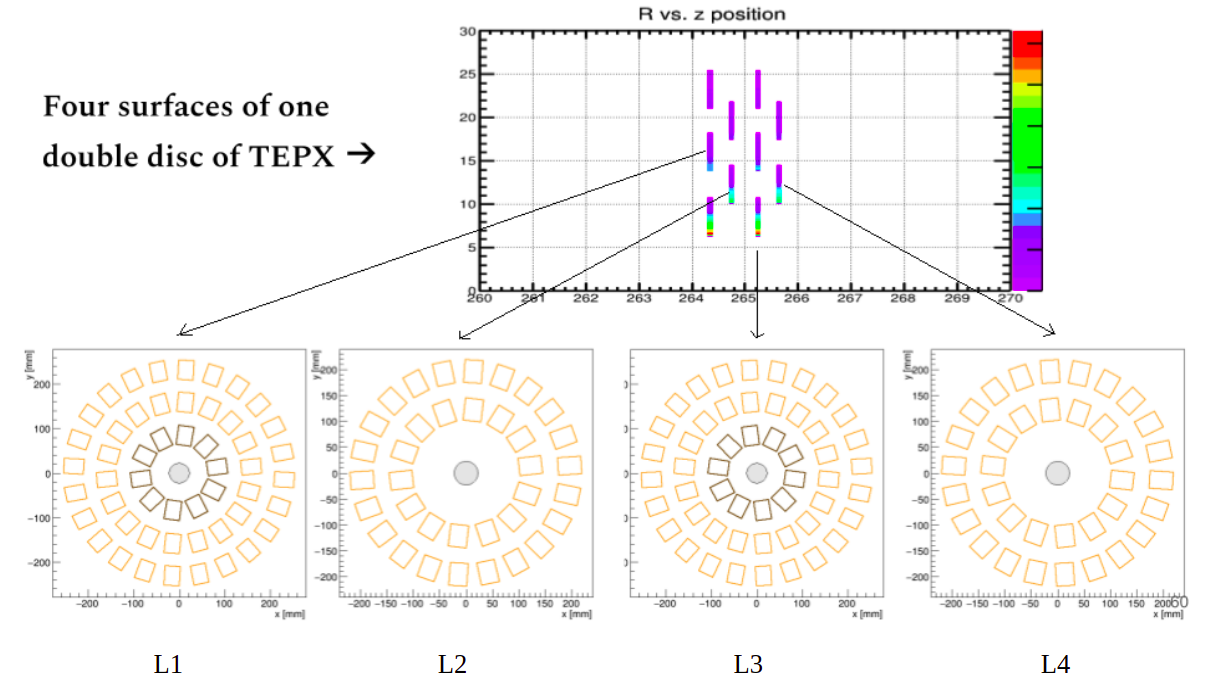
\includegraphics[width=1 \columnwidth]{./fourlayers.png}
  \caption{ \onehalfspacing Fours layers of one double disk of TEPX showing module arrangement in rings for each layer. Ring 1, 2, 3, 4 and 5 consists of 20, 28, 36, 44 and 48 modules respectively. }
  \label{fig:CMS}
\end{figure}

\subsection{Phase II CMS simulation samples}

\onelinespacing Simulated data samples for Phase II include full CMS detector description and uses official CMS software (CMSSW) version $10-6-0-patch2$ which calls GEANT4 for particle and energy deposit simulation as well as for reconstruction \cite{Agostinelli:2002hh}. These samples contain single-neutrino event overlaid with a variable number of minimum-bias events (events with any amount of real energy detected in CMS) to simulate different pileup values. The statistics for samples with average pileup values from 0.5 to 2 is 500000 events per step and for average pileup values between 10 and 200, statistics is 100000. \\

\subsection{Luminosity determination using TEPX - counting clusters/coincidences}

Instantaneous luminosity determination using PCC method for Phase II HL-LHC will be based on counting the number of clusters in TEPX Disk 4 Ring 1. The innermost ring of the last disk of TEPX (D4R1) is located at 2.65 m away from the interaction point that is beyond the tracking acceptance ($|\eta| = 4$) and as this region has few tracking points, it can be solely used for the purpose of luminosity measurement by using the full available trigger rate and bandwidth.\\

A new algorithm for luminosity determination based on counting two fold coincidences is proposed that applies selections using dr and $d\phi$ variables to minimize non-linearity for high pileup values as these variables take into account track angle and its curvature. Two fold coincidences are those hits which are created by the module overlap regions between various layers of one TEPX double disk. Two fold coincidences are better way to distinguish between a real hit and random electrical noise. They are more likely to be real hit than random electrical noise. Two fold coincidence in $\phi$ will involve modules overlapping in the same ring in front and back layers of one double disk as shown in top part of Fig. 27 and Fig. 28 while two fold coincidence in r will require modules overlapping between successive rings in the front (L1 $\&$ L2) and back layers (L3 $\&$ L4) of one double disk as shown in bottom part of Fig. 27. Luminosity calculated based on counting coincidences has an advantage over clusters that afterglow effects are tiny in the case of coincidences  \cite{Collaboration:2706512} \cite{brilsim} \cite{brilsim1}\cite{brilsim2}.\\



\begin{figure}[H]
  \centering
  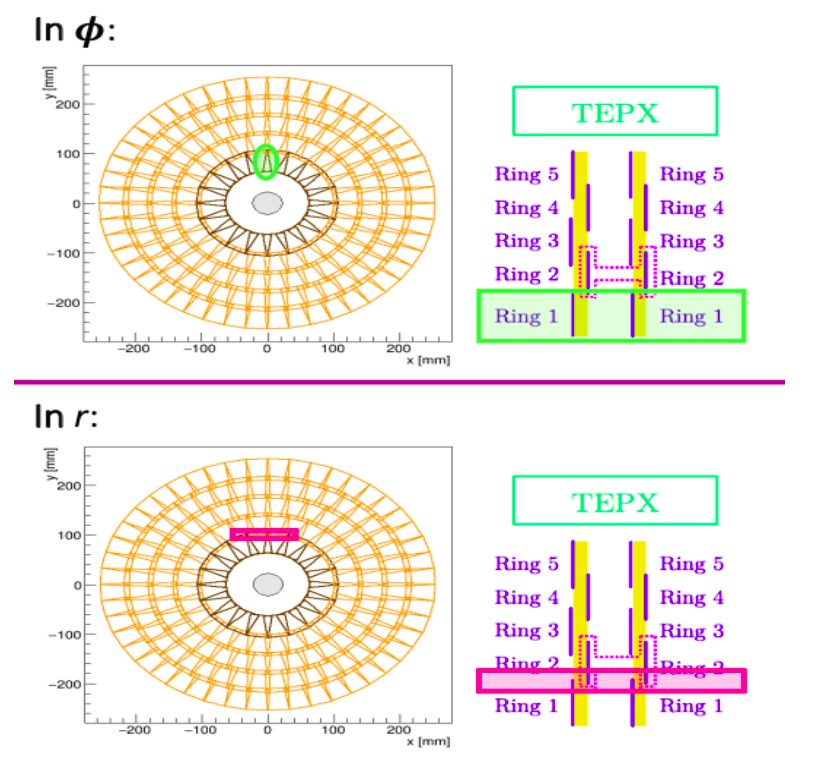
\includegraphics[width=0.7\columnwidth]{./2foldinrphi.png}
  \caption{ \onehalfspacing Diagram showing modules overlap between the front (L1 \& L2) and back (L3 \& L4) layers of one double disk of TEPX that creates two fold coincidences in $\phi$ and r.}
  \label{fig:CMS}
\end{figure}

\begin{figure}[H]
  \centering
  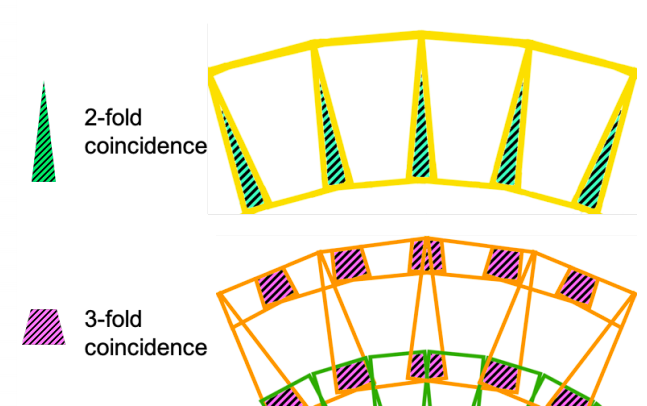
\includegraphics[width=0.6\columnwidth]{./23coin.png}
  \caption{\onehalfspacing Example of two and threefold coincidence regions on a portion of a single TEPX disk.}
  \label{fig:CMS}
\end{figure}

\subsection{TEPX linearity}

Linearity is one of the systematic uncertainty in the calculation of instantaneous luminosity and PCC visible cross section $\sigma_{vis}$. A linear relation between the number of clusters and pileup (PU) imply that \\

$<N_{cl/pp}> = \frac{<N_{cl}>}{\mu} = \frac{\sigma_{vis}}{\sigma_{pp}}$ \\

$<N_{cl}> =  \frac{\sigma_{vis}}{\sigma_{pp}} \mu $ \\

Linearity indicates that the PCC visible cross section $\sigma_{vis}$ does not depend on the per bunch instantaneous luminosity (ideal luminometer). In ideal scenario, $\sigma_{vis}$ is not dependent on pileup, but this a potential problem with the luminometer. Linearity results for simulated TEPX clusters and coincidences from low to high pileup values are shown from Fig. 29 to Fig. 40. TEPX luminometer proposed for Phase II shows excellent linearity over entire pileup range. A non-linear relation $<N_{cluster}> = \alpha (PU)^{\gamma}, \gamma \neq 1$ would add non-linear terms in the rate equation $R = \sigma_{vis} L_{inst}$  and cause $\sigma_{vis}$ to vary with the per bunch instantaneous luminosity and pileup values.


\begin{figure}[H]
  \centering
  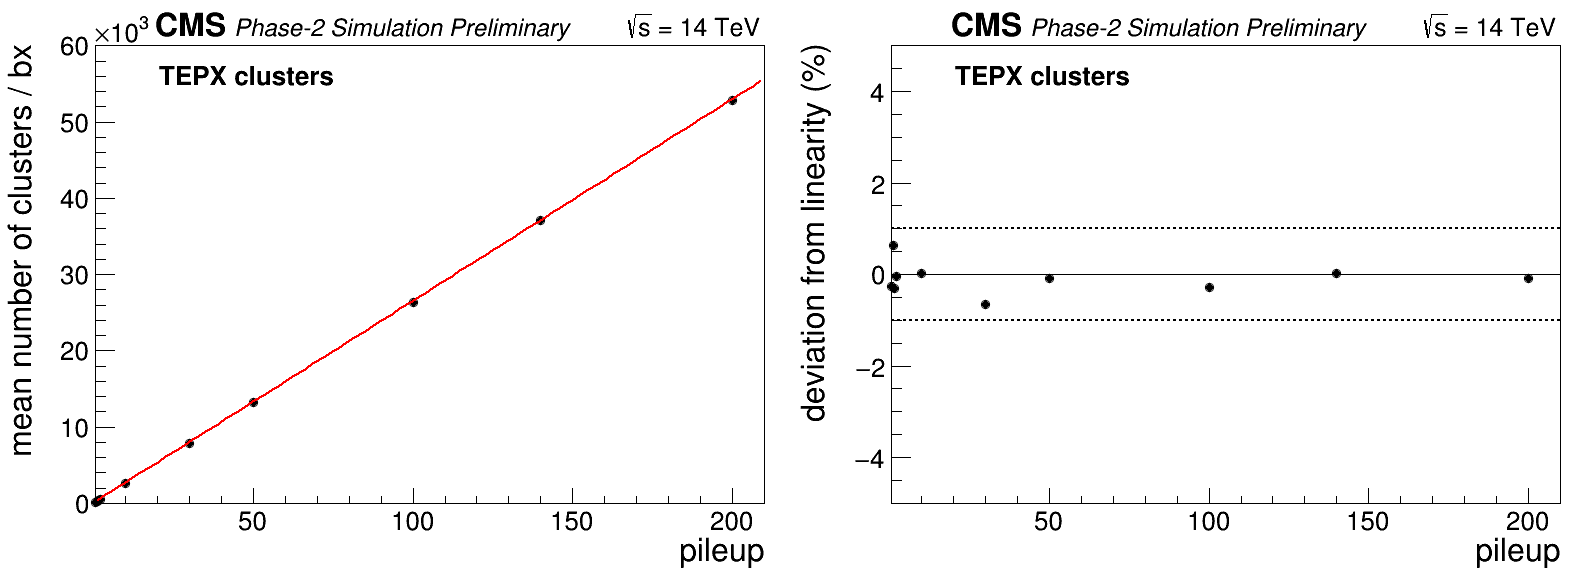
\includegraphics[width=1\columnwidth]{./totalclusters.png}
  \caption{\onehalfspacing Left: Simulated mean number of clusters for all entire TEPX detector as a function of pileup. A line is fitted between pileup values of 0 and 2, and then extrapolated up to a pileup of 200. Right: Deviation from linearity for clusters for entire TEPX detector. The non-linearity is calculated as the relative difference between the data points and the values of the fit function at the respective pileup value. Non-linearity is within 1 \% for entire pileup range. Pileup 200 corresponds to High Luminosity (HL)-LHC environment.}
  \label{fig:CMS}
\end{figure}



\begin{figure}[H]
  \centering
  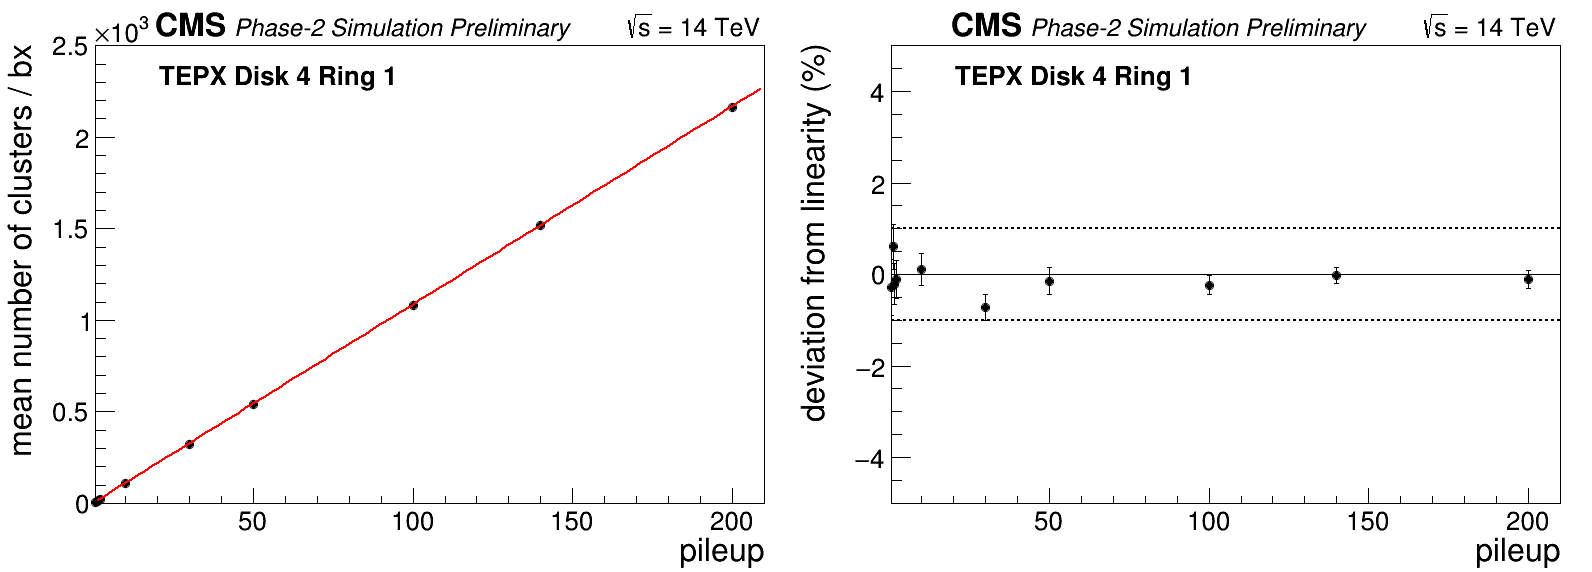
\includegraphics[width=1\columnwidth]{./clustersD4R1.png}
  \caption{\onehalfspacing Left: Simulated mean number of clusters for TEPX Disk 4 Ring 1 as a function of pileup. Right: Deviation from linearity for clusters for TEPX Disk 4 Ring 1. The non-linearity is calculated as the relative difference between the data points and the values of the fit function at the respective pileup value.}
  \label{fig:CMS}
\end{figure}



\begin{figure}[H]
  \centering
  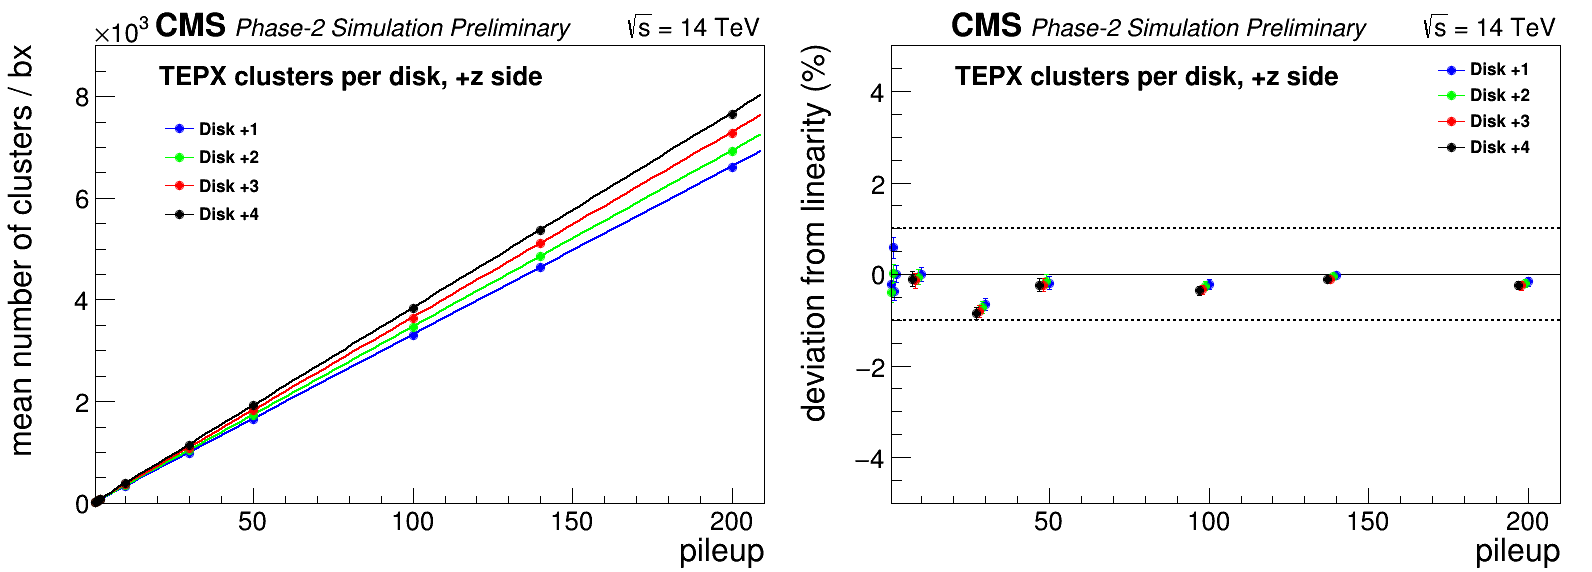
\includegraphics[width=1 \columnwidth]{./clustersperdisk+z.png}
  \caption{Left: Simulated mean number of clusters for +z side TEPX disks as a function of pileup. Right: Deviation from linearity for clusters for +z side TEPX disks.}
  \label{fig:CMS}
\end{figure}




\begin{figure}[H]
  \centering
  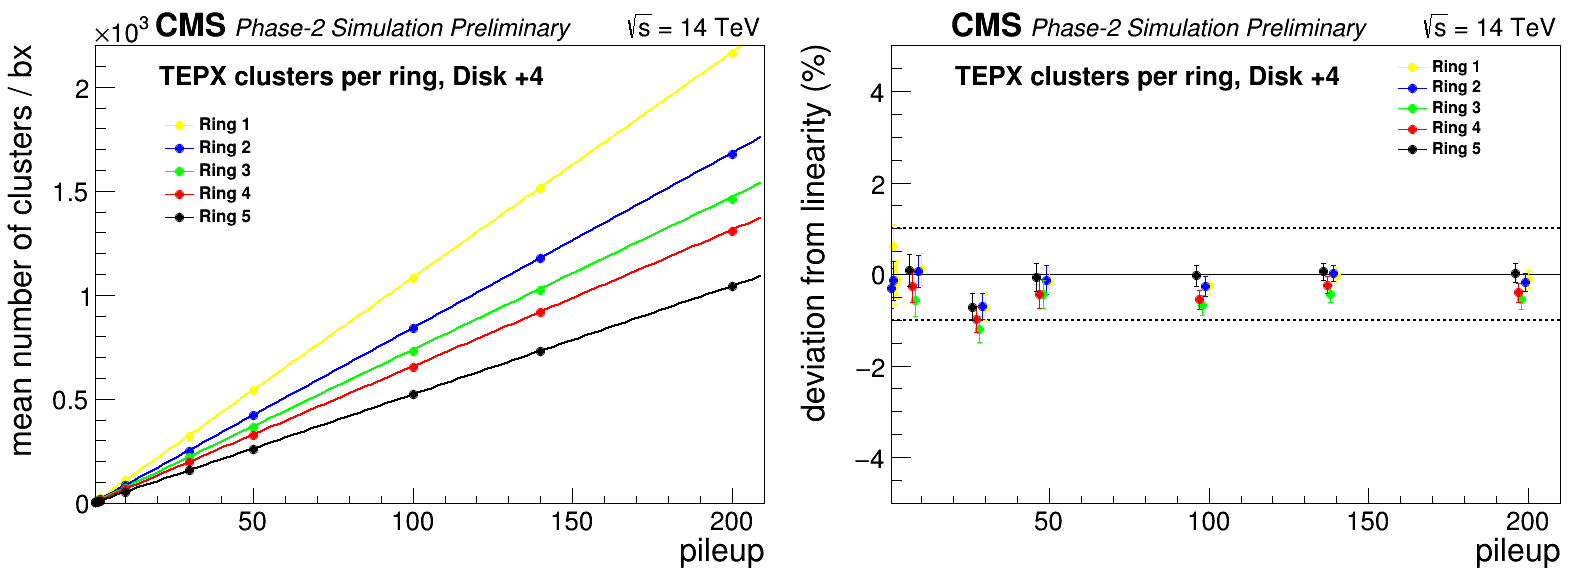
\includegraphics[width=1\columnwidth]{./clustersperringD+4.png}
  \caption{Left: Simulated mean number of clusters for +z side TEPX Disk 4 all rings as a function of pileup. Ring 1 has highest slope and Ring 5 has least slope. Right: Deviation from linearity for clusters for TEPX Disk +4 all rings. Non-linearity is within $1\%$ for all rings over entire pileup range.}
  \label{fig:CMS}
\end{figure}


\begin{figure}[H]
  \centering
  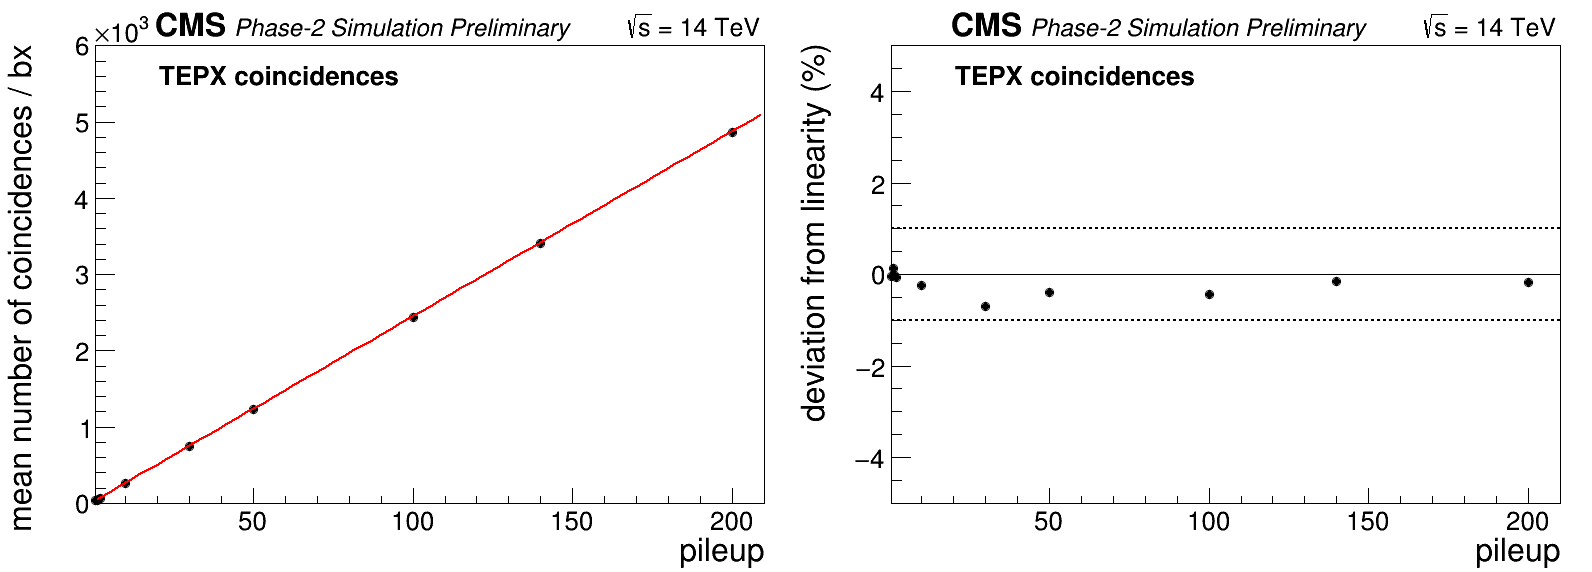
\includegraphics[width=1 \columnwidth]{./totalcoincidences.png}
  \caption{Left: Simulated mean number of coincidences in $\phi$ and r for all entire TEPX detector as a function of pileup. A line is fitted between pileup values of 0 and 2, and then extrapolated up to a pileup of 200. Right: Deviation from linearity for coincidence in $\phi$ and r for entire TEPX detector. The non-linearity is calculated as the relative difference between the data points and the values of the fit function at the respective pileup value. Non-linearity is within 1 \% for entire pileup range. Pileup 200 corresponds to High Luminosity (HL)-LHC environment.}
  \label{fig:CMS}
\end{figure}


\begin{figure}[H]
  \centering
  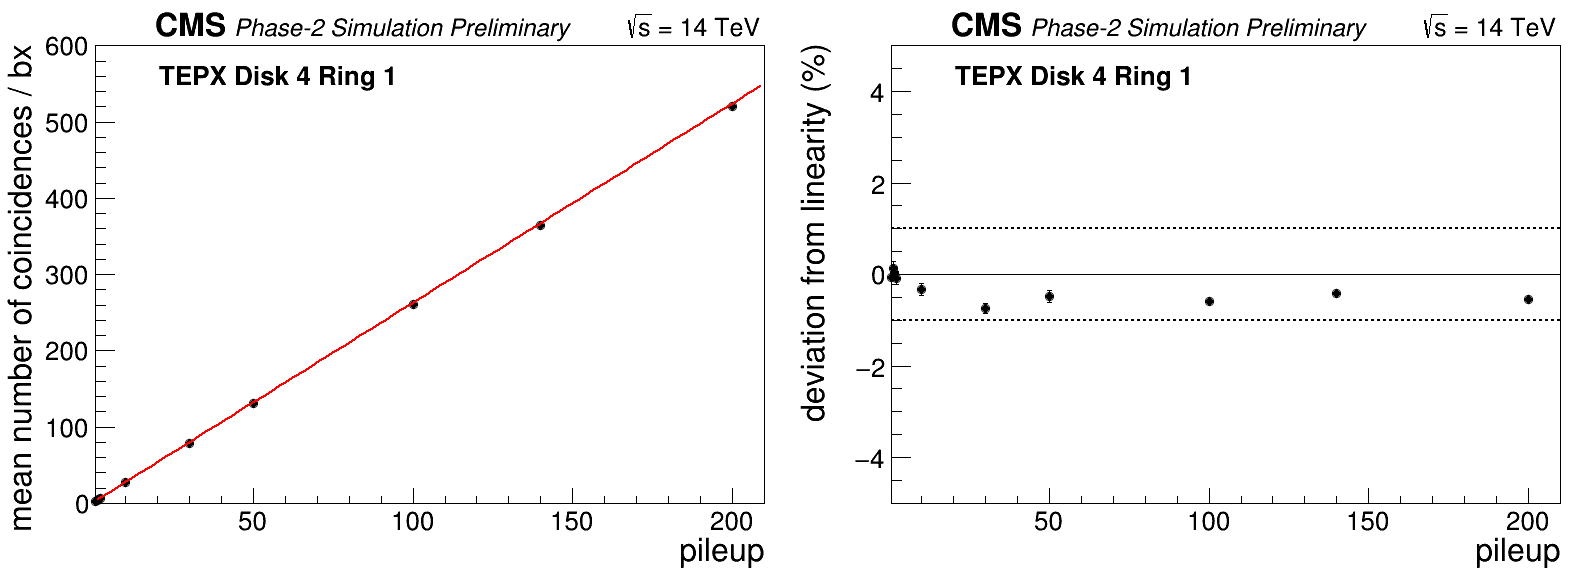
\includegraphics[width=1\columnwidth]{./totalcoincidencesD4R1.png}
  \caption{Left: Simulated mean number of coincidences in $\phi$ and r for TEPX Disk 4 Ring 1 as a function of pileup. Right: Deviation from linearity for coincidences in $\phi$ and r for TEPX Disk 4 Ring 1. The non-linearity is calculated as the relative difference between the data points and the values of the fit function at the respective pileup value.}
  \label{fig:CMS}
\end{figure}





\begin{figure}[H]
  \centering
  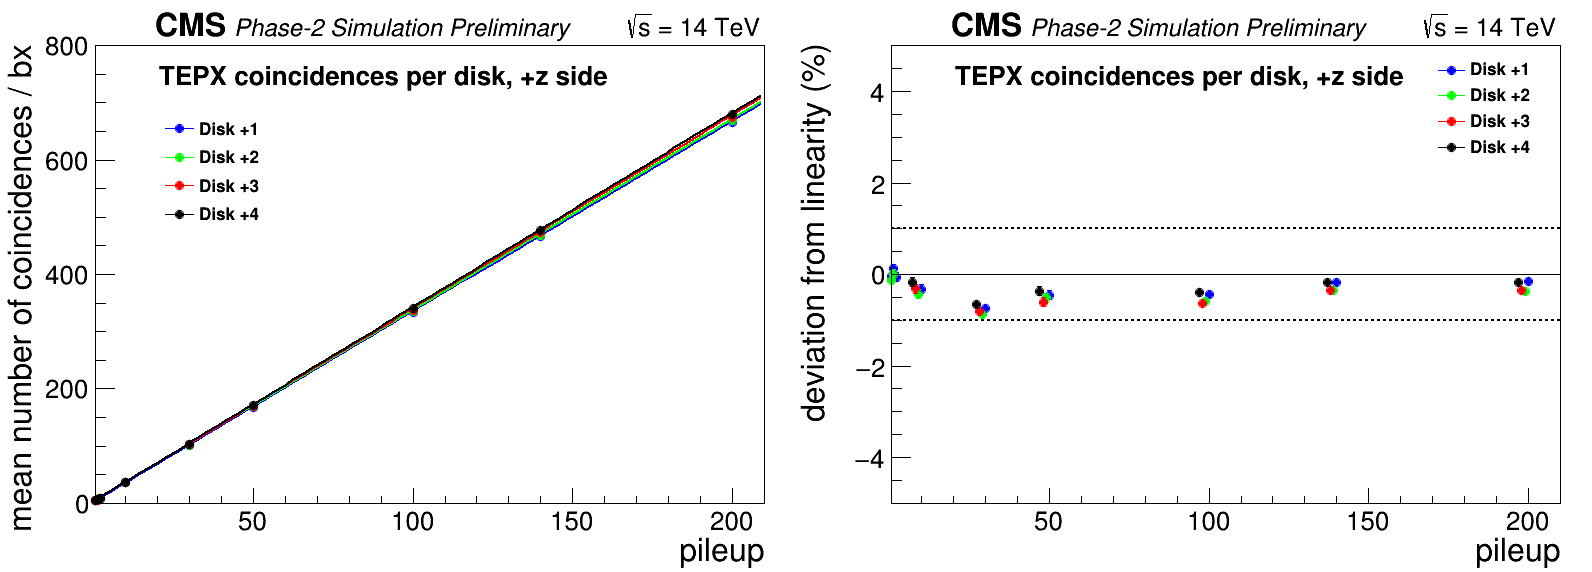
\includegraphics[width=1\columnwidth]{./coincidencesperdisk+z.png}
  \caption{Left: Simulated mean number of coincidences in $\phi$ and r for +z side TEPX disks as a function of pileup. Right: Deviation from linearity for coincidences in $\phi$ and r for +z side TEPX disks.}
  \label{fig:CMS}
\end{figure}


\begin{figure}[H]
  \centering
  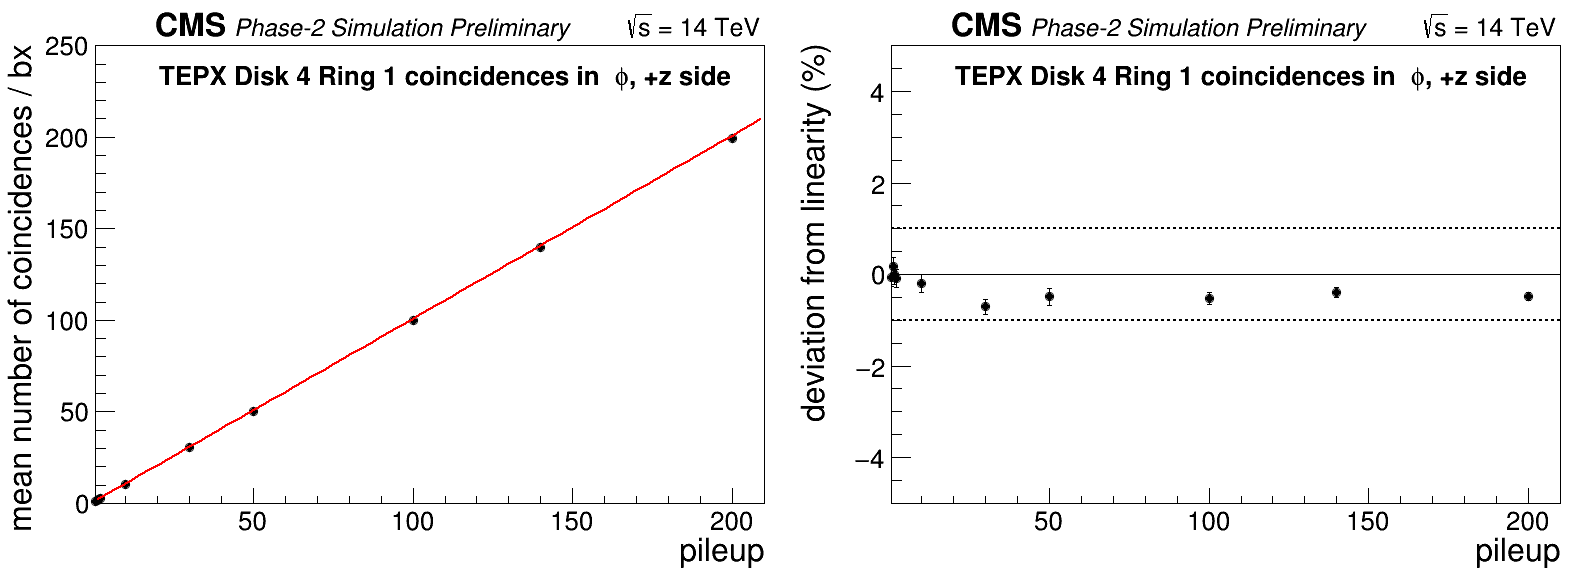
\includegraphics[width=1\columnwidth]{./coincidencesinphiD4R1z+.png}
  \caption{Left: Simulated mean number of coincidences in $\phi$ for TEPX +z side Disk 4 Ring 1 as a function of pileup. Right: Deviation from linearity for coincidences in $\phi$ for TEPX +z side Disk 4 Ring 1. The non-linearity is calculated as the relative difference between the data points and the values of the fit function at the respective pileup value.}
  \label{fig:CMS}
\end{figure}



\begin{figure}[H]
  \centering
  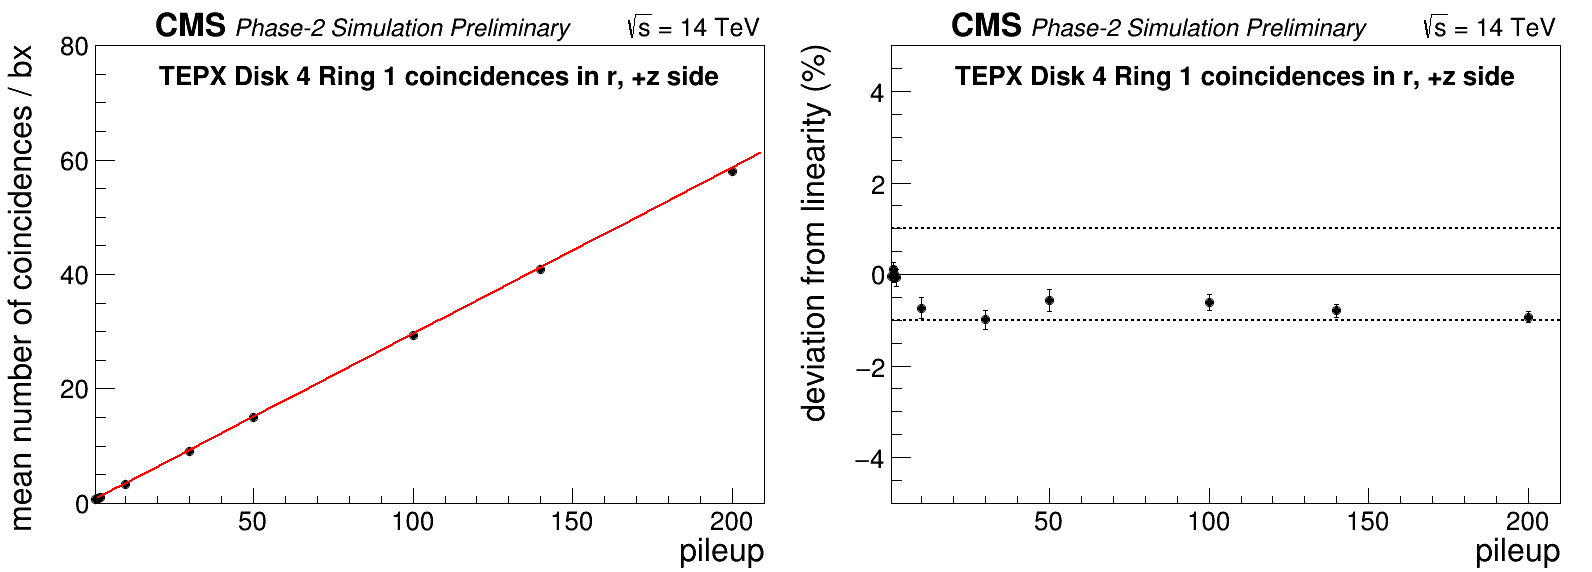
\includegraphics[width=1\columnwidth]{./coincidencesinrD4R1z+.png}
  \caption{Left: Simulated mean number of coincidences in r for TEPX +z side Disk 4 Ring 1 as a function of pileup. Right: Deviation from linearity for coincidences in r for TEPX +z side Disk 4 Ring 1. The non-linearity is calculated as the relative difference between the data points and the values of the fit function at the respective pileup value.}
  \label{fig:CMS}
\end{figure}





\begin{figure}[H]
  \centering
  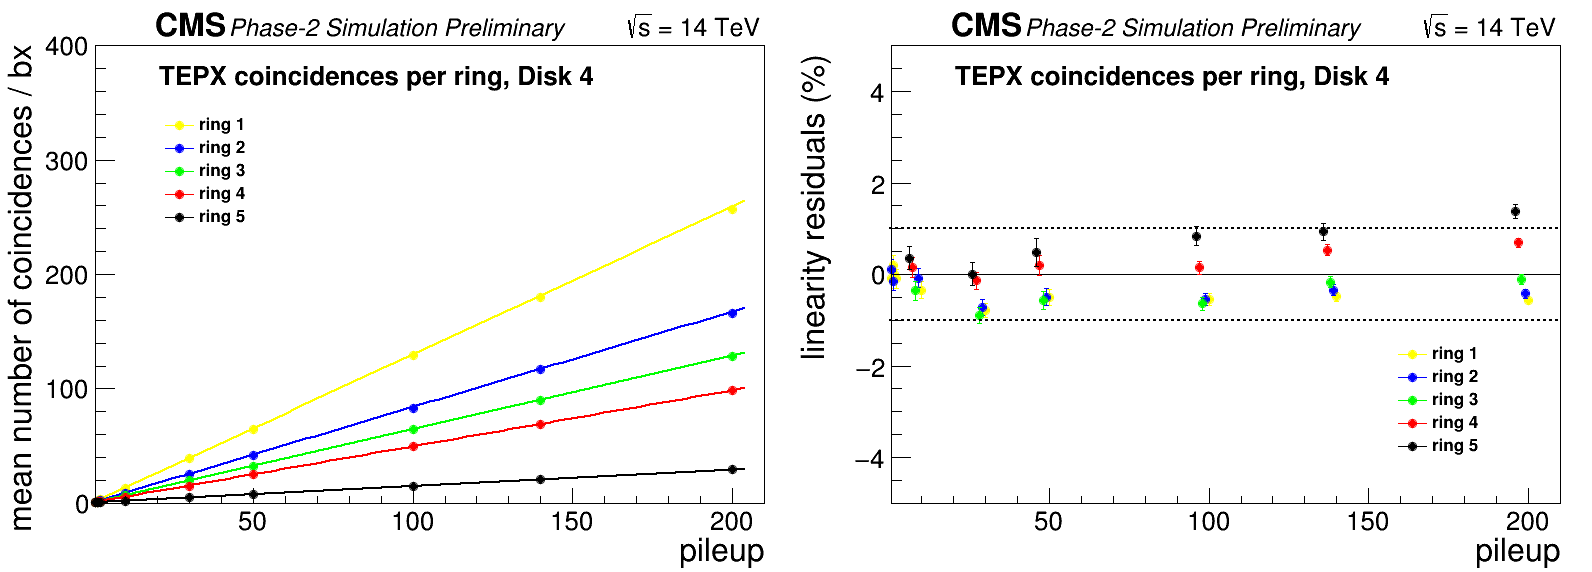
\includegraphics[width=1\columnwidth]{./coincidencesperringD+4.png}
  \caption{Left: Simulated mean number of coincidences in $\phi$ and r for +z side TEPX Disk 4 per ring as a function of pileup. Ring 1 has highest slope and Ring 5 has least slope. Right: Deviation from linearity for coincidences in $\phi$ and r for +z side TEPX Disk 4 per ring. Non-linearity is within 1\% for all rings over entire pileup range.}
  \label{fig:CMS}
\end{figure}








\begin{figure}[H]
  \centering
  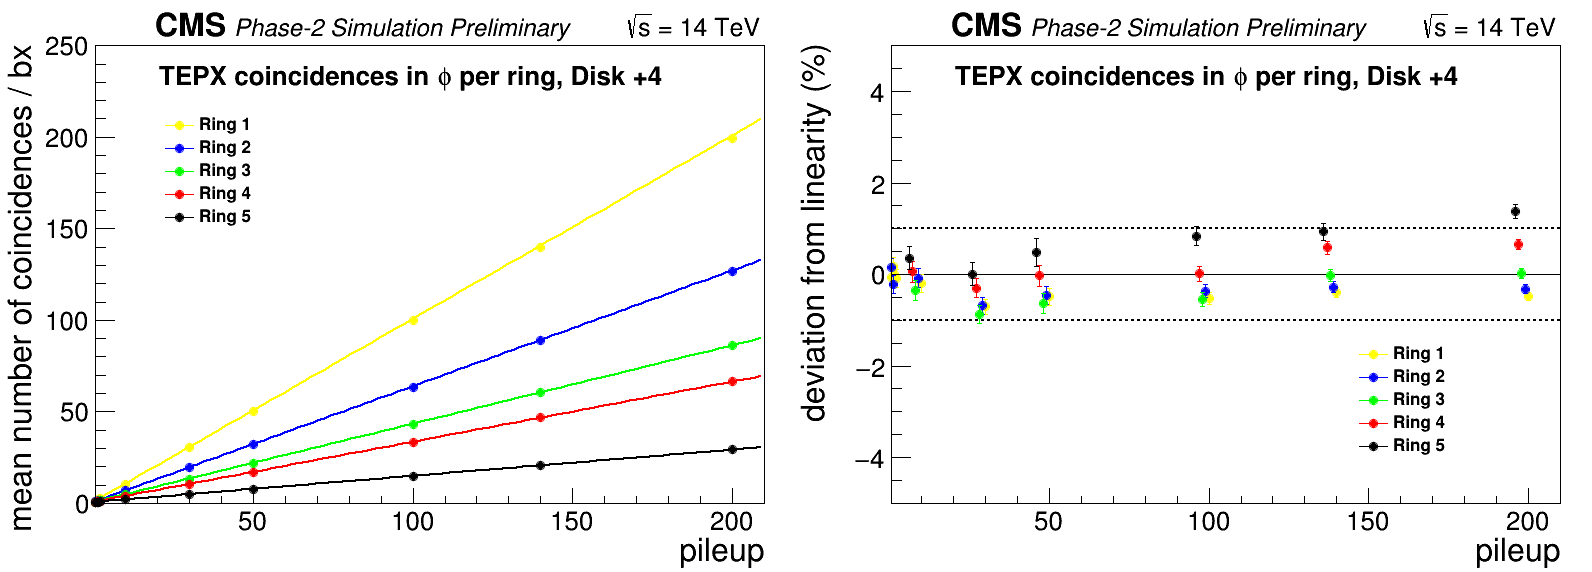
\includegraphics[width=1\columnwidth]{./coincidencesinphiperringD+4.png}
  \caption{Left: Simulated mean number of coincidences in $\phi$ for +z side TEPX Disk 4 per ring as a function of pileup. Ring 1 has highest slope and Ring 5 has least slope. Right: Deviation from linearity for coincidences in $\phi$ for +z side TEPX Disk 4 per ring. Non-linearity is within 1\% for all rings over entire pileup range.}
  \label{fig:CMS}
\end{figure}





\begin{figure}[H]
  \centering
  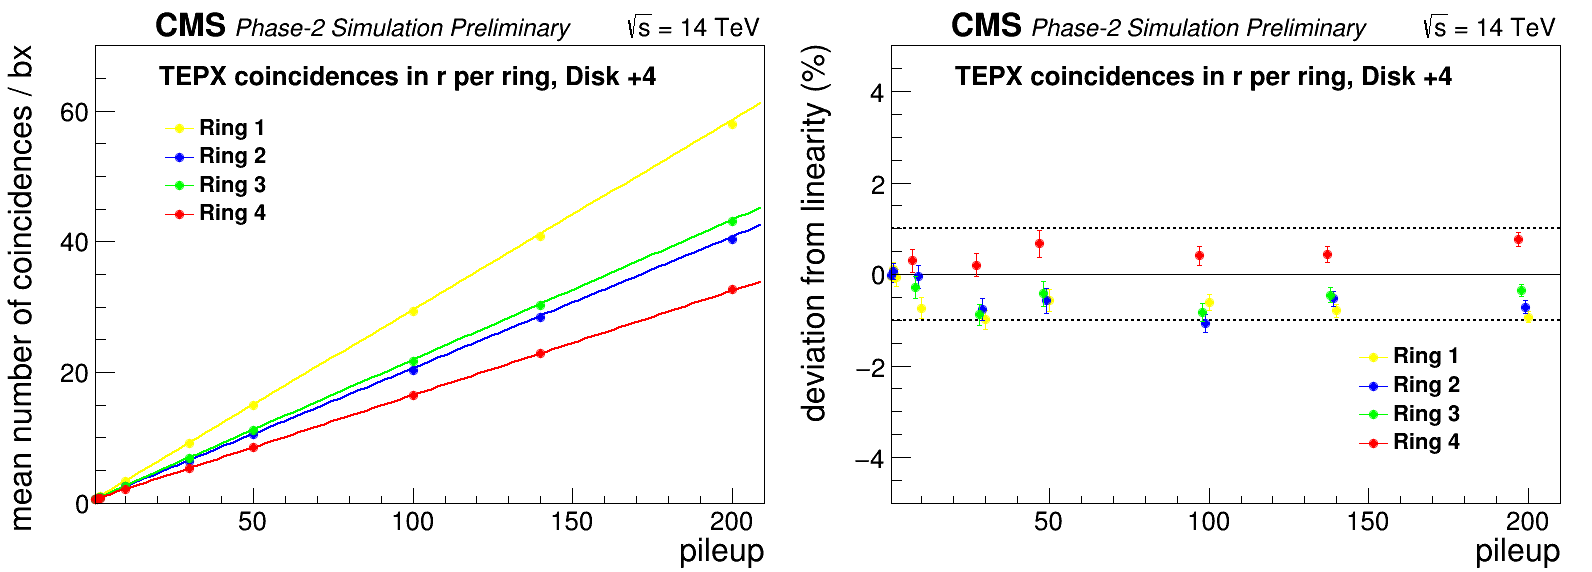
\includegraphics[width=1\columnwidth]{./coincidencesinrperringD+4.png}
  \caption{Left: Simulated mean number of coincidences in r for +z side TEPX Disk 4 per ring as a function of pileup. Ring 1 has highest slope and Ring 5 has least slope. Right: Deviation from linearity for coincidences in r for +z side TEPX Disk 4 per ring. Non-linearity is within $1\%$ for all rings over entire pileup range.}
  \label{fig:CMS}
\end{figure}


\subsection{Statistical precision for TEPX luminometer}
Statistical precision is another uncertainty that need to be considered for precise luminosity measurement. It must be kept minimal to achieve 1 $\%$ accuracy for HL-LHC luminosity measurement. \\

Relative statistical uncertainty in $\%$ = $\frac{\sqrt{N}}{N} \times 100$ \\

where N = (Number of counts per event)$\times$(Trigger Frequency)$\times$(Time Integration period). \\

\newpage

\clearpage\newpage

\begin{flushleft} 
Table 1: Expected statistical precision (in $\%$) in head-on collisions during typical vdM conditions with pileup of 0.5 for TEPX clusters and two fold coincidences over different integration time period.
\end{flushleft} 
\begin{center}
\scalebox{1}{
\begin{tabular}{|l | c | c | c |c|}
\hline
 vdM (PU 0.5) & Readout Rate (kHz) &1 bx, 1s & 1 bx, 30s & 100 bx, 30s\\
\hline
TEPXD4R1 Clusters&1000&1.82&0.332 & 0.0332\\
\hline
TEPXD4R1 2x Coincidences in phi &1000&5.98&1.09 & 0.109\\
\hline
TEPXD4R1 2x Coincidences in r &1000&11.1&2.02 & 0.202\\
\hline
TEPXD4R1 2x Coincidences &1000&5.27&0.962 & 0.0962\\
\hline
TEPX Clusters&500&0.709&0.129 & 0.0129\\
\hline
TEPX 2x Coincidences in phi &500&2.65&0.485 & 0.0485\\
\hline
TEPX 2x Coincidences in r &500&4.59&0.838 & 0.0838\\
\hline
TEPX 2x Coincidences &500&2.3&0.42 & 0.042\\
\hline
\end{tabular}}
\end{center}

\begin{flushleft} 
  Table 2: Expected statistical precision (in $\%$) in head-on collisions during physics conditions with pileup of 200 for TEPX clusters and two fold coincidences over different integration time period.
  \end{flushleft} 
\begin{center}
\scalebox{1}{
\begin{tabular}{|l | c | c | c |c |}
\hline
Algorithm & Readout Rate (kHz)& 1 bx, 1s &2500 bx, 1s   & 2500 bx, 1 LS \\
\hline
TEPXD4R1 Clusters&825&0.1&0.002&0.000414\\
\hline
TEPXD4R1 2x Coincidences in phi &825&0.329&0.00659&0.00136\\
\hline
TEPXD4R1 2x Coincidences in r &825&0.61&0.0122&0.00252\\
\hline
TEPXD4R1 2x Coincidences  &825&0.29&0.0058&0.0012\\
\hline
TEPX Clusters &75&0.0915&0.00183&0.000379\\
\hline
TEPX 2x Coincidences in phi &75&0.343&0.00685&0.00142\\
\hline
TEPX 2x Coincidences in r &75&0.593&0.0119&0.00245\\
\hline
TEPX 2x Coincidences &75&0.297&0.00594&0.00123\\
\hline
\end{tabular}}
\end{center}

\newpage

